\subsection{Guidance, Navigation, and Control Software} \label{GNC_Software}
\noindent The block titled "invoke GNC software loop" seen in figure \ref{fig:Polite-Mobile-Obstacle-Avoidance-Flowchart} is a key part of our system. This code must take in all of our sensor data and make calculated decisions to avoid said hazards, and it must do so in real time and then guide the system according to these decisions. We have the ability to poll our sensor data as needed through the use of the functions we have developed in our code. Thus, we will use this data to assess the current environment, make a decision to move out of the way of the hazard, and loop this at four Hertz (every 250 milliseconds) until we have determined an all clear signal. We will then guide the user back to their initial path through the IMU data, mainly the yaw angle that we will capture prior to beginning this loop. \\
\noindent The diagram seen in figure \ref{fig:Polite-Mobile-Obstacle-Avoidance-Flowchart} illustrates the software logic flow for our system. \\

\begin{figure}[H]
	\centering
	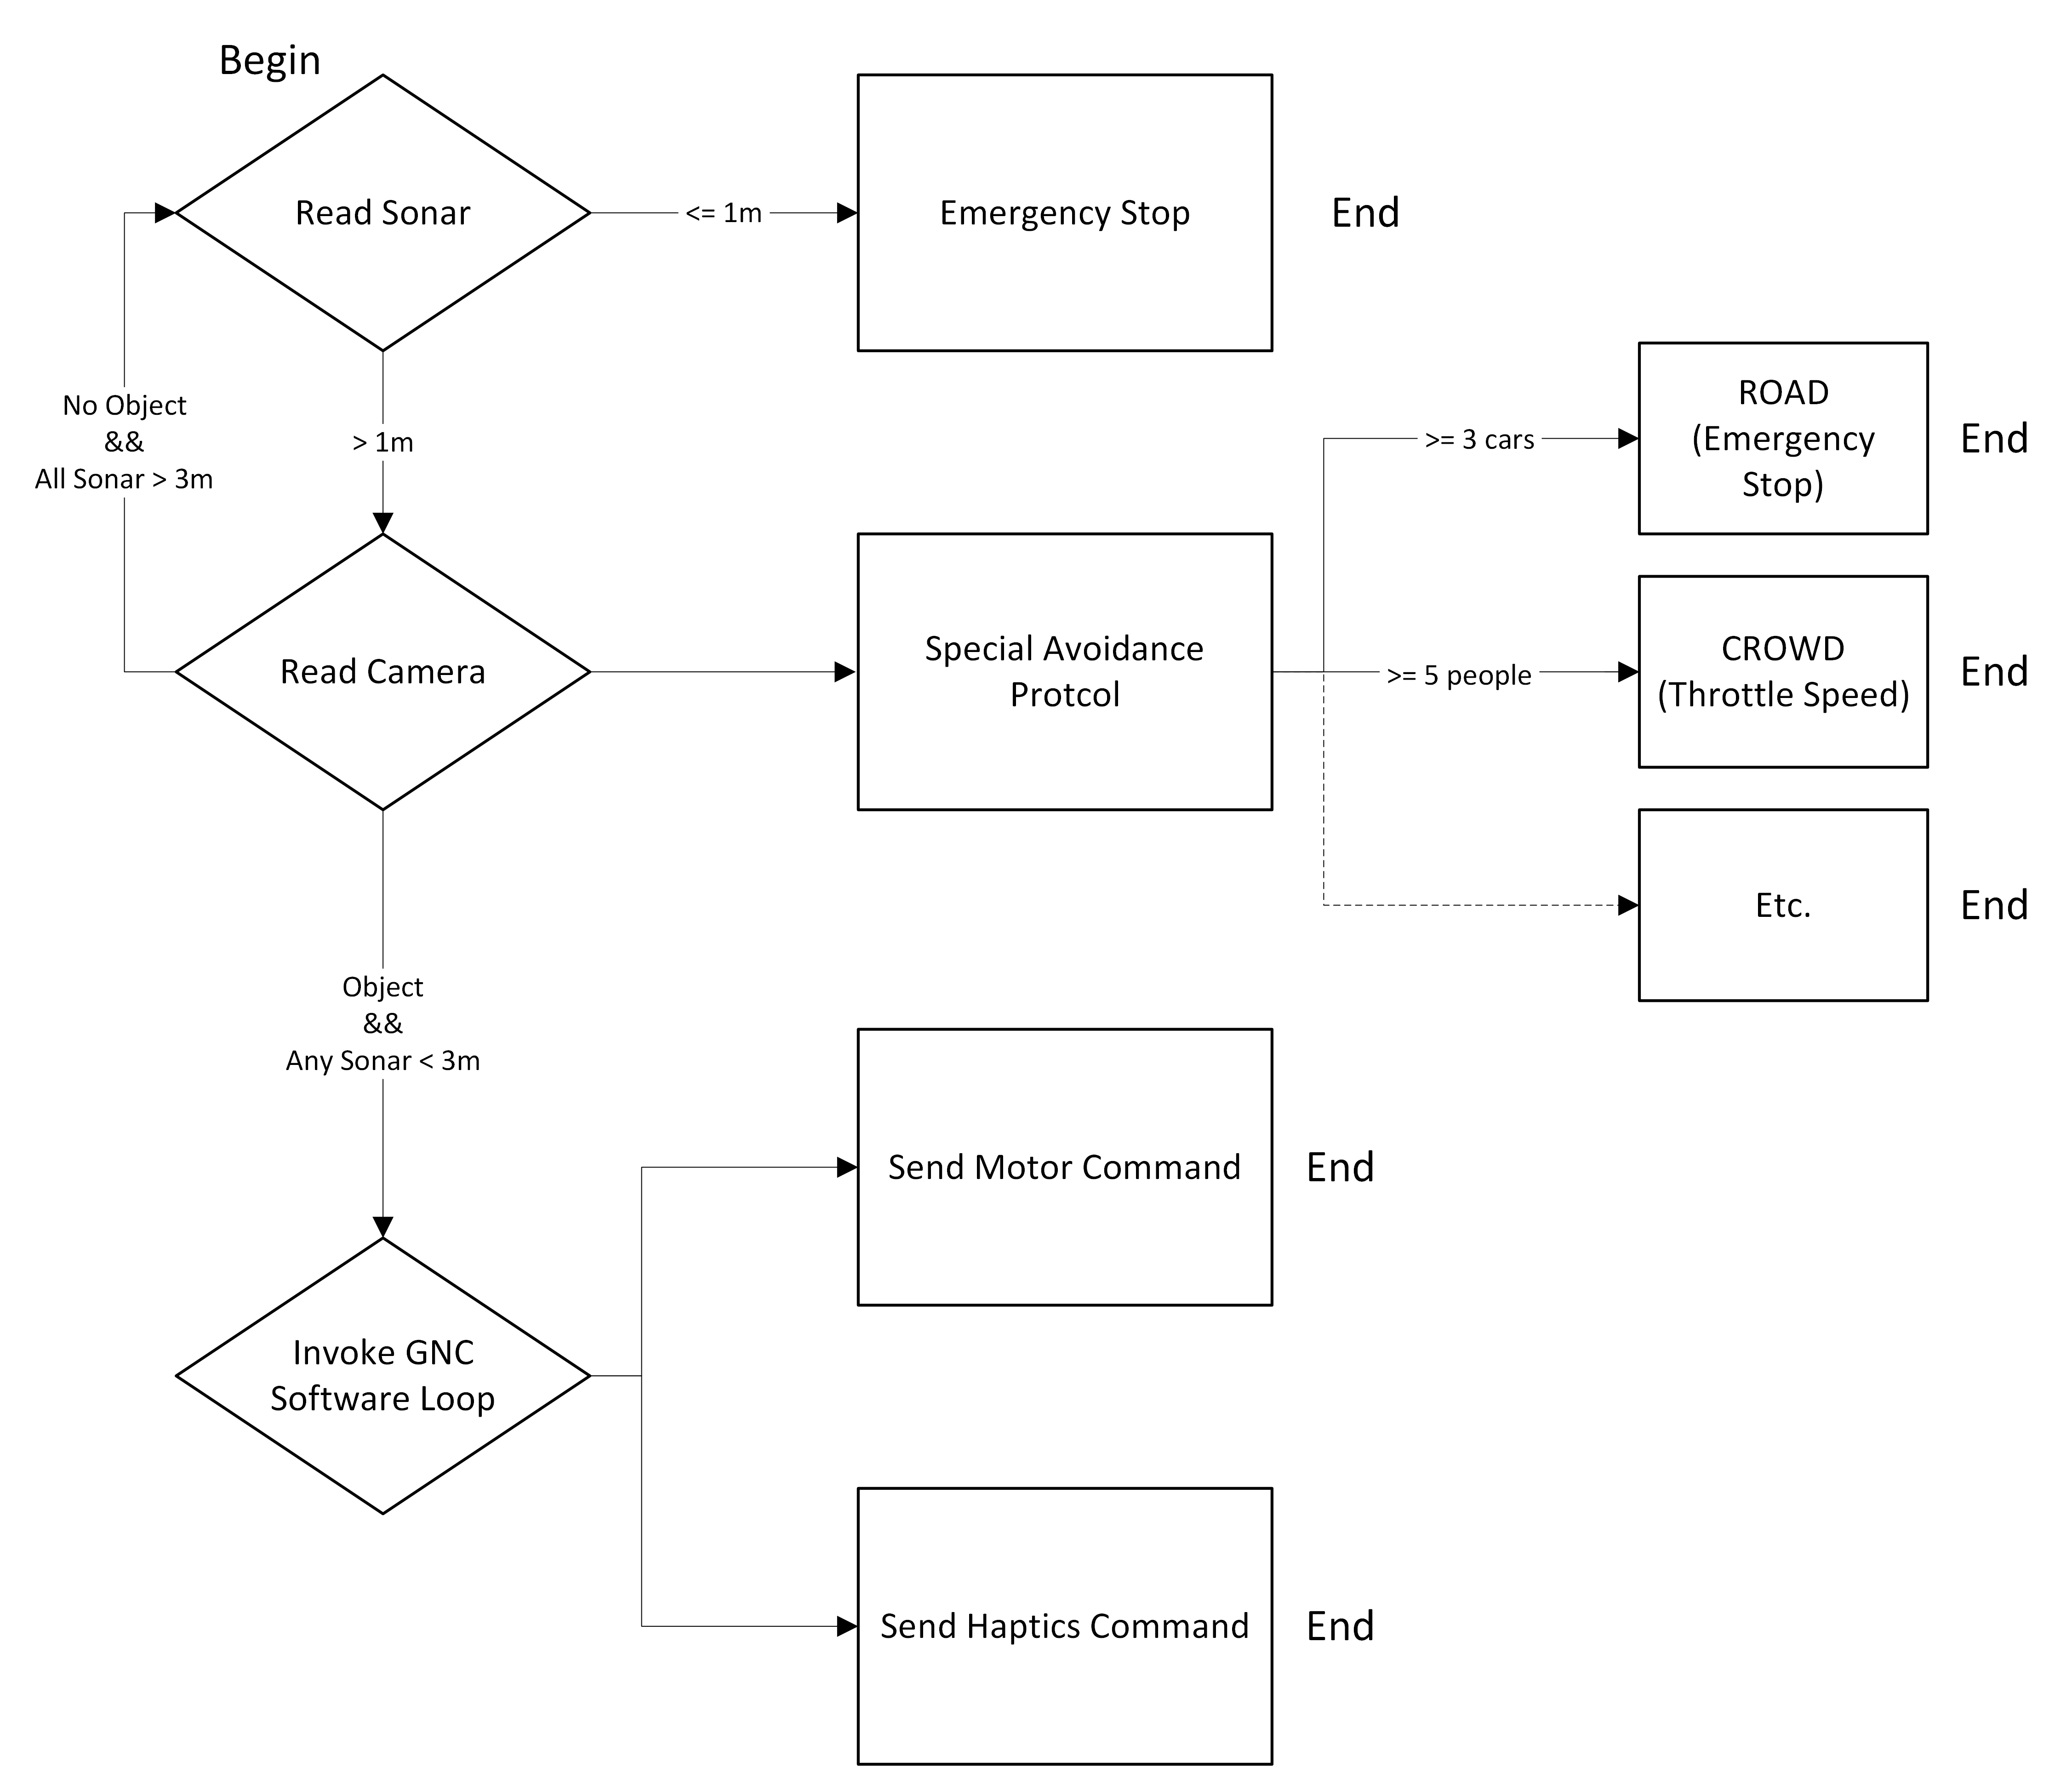
\includegraphics[width=1.0\textwidth]{./Images/Polite-Mobile-Obstacle-Avoidance-Flowchart.png}
	\caption{\label{fig:Polite-Mobile-Obstacle-Avoidance-Flowchart}Polite Mobile Obstacle Avoidance Flowchart}
\end{figure}

\noindent The flowchart begins at processing the Sonar sensor readings. These readings are done first due to their relatively low latency and accuracy for determining if we are in need of an immediate stop. We then continue onward to the camera readings if we have a sonar reading greater then one meter. In the camera stage, we continue looping if all sonar readings are outside of three meters and no object has been detected - this loop indicating a clear walk zone for the system. We also check certain conditions for specific avoidance protocols, such as more then three cars indicating a parking lot or road, or more then five people indicating a large crowd, but as long as these aren't met, and the loop condition is meet, our system will continue moving as normal. When we read either an sonar less then three meters or detect an object in our camera, we then invoke our GNC software loop and guide the system out of harms way and back to their path. The GNC software outputs commands to the motors in real time to alert the user via haptics and guide the system via Dc brush motors. The GNC software loop is discussed in greater detail below in section \ref{GNC_Software}. \\


\noindent [TOBYBOT GET IN HERE CHIEF KEEF] \\
\noindent GNC situation, tilt (attitude) using IMU, (incline decline), velocity and position solutions, ESP32 source code GitHub (hc-sr04.c luna.c haptic.c audio.c motor.c ip.c avoid.c), motor commands calculation. \\

\subsection{Object Detection}
\noindent The computer vision aspect of our software is very straight forward. The Arduino IDE contains example code for each board file and has an example of an object detection algorithm for the AMB82-MINI board. To implement this for our purposes, we maintained the YOLO4 Tiny model configuration, the already existing class list for the objects to be detected, and the main loop to extract this data from the algorithm. \\

\noindent While we were able to utilize the example code to help in getting started, there was additional functionality needed to properly fit our purposes. The first of these was implementing WiFi and UDP communication on the board. After doing such, we used a while loop to wait for the ESP32 to assert a transmit flag and once received, the AMB82-MINI board would complete an object detection run and transmit the data to the ESP32. We also will perform later testing to determine which model and which of the objects in the object list class are most effective for our purposes, aiming to decrease latency and increase accuracy. \\

\noindent GNC situation, tilt (attitude) using IMU, (incline decline), velocity and position solutions, ESP32 source code GitHub (hc-sr04.c luna.c haptic.c audio.c motor.c ip.c avoid.c), motor commands calculation\\

tracking moving obstacle\\

navigation is all done by the IMU\\

guidance algorithm\\

control actuation code\\  

\noindent [UML CLASS DIAGRAM HERE]\\

\subsection{Computer Vision}
\noindent For this section, another stretch goal that we plan to attempt to implement, is the functionality to detect walls, grass, and other constantly colored objects that have a difficult time being classified in our detection system. To do this we will implement a color sensor, either through the on board camera, or through an external color sensor such as the TCS34725 to pull the raw RGB data values, make comparisons, and then pass the data along. \\

\noindent This could be particularly useful for avoiding grassy terrain, which will cause greater risk to the user as well as large unavoidable objects such as walls, which can be dangerous and halt movement altogether. The risk in implementing this functionality will be the confidence of our predictions as well as the danger of mispredictions, but overall, we expect to increase FORWARD's ability to effectively and safely navigate the user through day to day life. \\


\subsection{Serial Interfaces}
\noindent As discussed in section \ref{ardumatlab}, we can port the serial plotter data for the ranges and IMU to MATLAB in order to visualize the field of view. See equation \ref{Polar}. We can visualize obstacles present because of dips in the range outputs. We also can visualize attitude and orientation based on IMU outputs. Putting these into MATLAB plots will provide valuable insight into the dynamics of the entire system as it traverses a test environment. It also interfaces between non-visual and visually based sensing methods by creating a map of the environment.\\

\noindent Mathematically, we know that the \underline{\textit{navigational plane}} is two-dimensional, with the reference frame origin located at the rollator center of mass. The positive x-axis is forward looking aft, the positive y-axis is left facing aft, and the positive z-axis is vertically upward. Because of the 2D nature, we can negate the z-axis because we do not sense altitude, nor is FORWARD an airborne system. It always stays grounded. Therefore, the guidance commands are given to the yaw angle (x-axis orientation) and the motor speed, which is actuated when on an incline or decline as shown in \ref{fig:slope-stability}. In essence, based on obstacles detected and classified, FORWARD will prompt the user to steer left or right. It should never prompt the user to go backwards or to travel vertically upward. The one exception is for curb lifting, which admittedly is a difficult maneuver to achieve: a stretch goal.\\